\documentclass[a4paper,11pt,openany]{memoir}
%
% AUTHOR: Nicolás Otero Martínez - nom05 (at) uvigo.es.
% COLLABORATORS: -
% MIT License in the corresponding file.
% This LaTeX code employs `memoir' class.
% Some code was used from:
%
\usepackage{mystyle}   %% Includes all packages

\newcommand\versionprog{1.2.17}
\newcommand\programa{\textsc{NDELOC}}

\hypersetup{
	pdfauthor={Nicol\'{a}s Otero Martínez},
	pdftitle={\programa~v\versionprog}
}

\addbibresource{biblio.bib}

\title{\programa~\versionprog: a program to compute multicenter electron delocalization indices}
\author{Nicol\'{a}s Otero Mart\'{i}nez, Marcos Mandado Alonso}
\date{\today}

\begin{document}
\acrodef{HI}{Hirsfeld-I}
\acrodef{HF}{Hartree-Fock}
\acrodef{KS}{Kohn-Sham}
\acrodef{DFT}{density functional theory}
\acrodef{FOHI}{fractional occupation \mbox{Hirsfeld-I}}
\acrodef{MO}{molecular orbital}
\acrodef{2-DI}{2-center delocalization index}
\acrodef{6-DI}{6-center delocalization index}
\acrodef{DI}{delocalization index}
\acrodefplural{DI}{delocalization indices}
\acrodef{GPA}{Generalized Population Analysis}
\acrodef{PAH}{polycyclic aromatic hydrocarbon}
\acrodef{QTAIM}{Quantum Theory of Atoms In Molecules}
\acrodef{ELF}{electron localization function}
\acrodef{SOS}{sum-over-states}
\acrodef{BSSE}{basis set superposition error}
\acrodef{FMR}{fragment of molecular response}
\acrodef{AOM}{atomic overlap matrix}
\acrodefplural{AOM}{atomic overlap matrices}
\acrodef{BOM}{basin overlap matrix}
\acrodefplural{BOM}{basin overlap matrices}
\acrodef{GPA}{Generalized Population Analysis}

\cleardoublepage \let\cleardoublepage\clearpage

\frontmatter % Front matter begins

\begin{titlingpage}

	\begin{center}
	
		\vspace{1cm}
		
		{\Huge\textbf{\programa~\versionprog}\\[.5cm]
				{\LARGE a Program to Compute Multicenter Electron Delocalization Indices}}
		
		\vspace{1cm}
		
		% Specify custom columns types with fixed width and left and right alignment
		\newcolumntype{x}[1]{%
		>{\raggedleft\hspace{0pt}}p{#1}}%
		\newcolumntype{y}[1]{%
		>{\raggedright\hspace{0pt}}p{#1}}%
		
		\hrule
		\vspace{.5cm}
		\begin{tabular}{x{6.5cm}y{4.5cm}}
		Author: & e-mail: \tabularnewline
		Nicol\'{a}s Otero Mart\'{i}nez & \url{nom05@uvigo.es} \tabularnewline
		Marcos Mandado Alonso & \url{mandado@uvigo.es} \tabularnewline
		\end{tabular}\\[.5cm]

		\hrule
		
		\vspace{7cm}
		
		\begin{center}
			\begin{tabular}{c@{\hspace{3cm}}c}
				Nicolás Otero Martínez & Marcos Mandado Alonso
			\end{tabular}
		\end{center}
		
		\vspace{0.5cm}
		
		\today
		
		\vfill
		
		
\includegraphics[width=9cm]{figures/logo}
	
	\end{center}

\end{titlingpage}

% The * after \tableofcontents prevents it from getting an entry in the TOC
\tableofcontents*

% Main matter begins
\mainmatter

%\begin{OnehalfSpace} % Use to begin double line spacing

\chapter{\programa~ scheme and software}

% Fixed width box
\nota{This document is a short guide to use \programa, a program developed as a parallelized computation of $N$-center electron (de)localization (localization and delocalization) indices, in which $N \ge 2$, and the ``centers'' represent atoms or regions obtained from a molecular real space partitioning (such as \acs{QTAIM}, \acs{ELF} and Hirshfeld-based approaches). These indices are currently employed as a criterion to study chemical challenges related to concepts like bond orders, pericyclic reactions, 3-center 2-electron bonds (such as the \ce{B2H6} ``banana bonds'') and, especially, aromaticity.}

\section{Scheme of the program}
\programa~ is a software designed to perform computations of multicenter (or $N$-center) electron localization and delocalization indices in a parallelized and efficient way from real space partitionings, such as \ac{QTAIM}\autocite{bader1994atoms}, \ac{ELF}\autocite{simplemeasureelectronBE1990,ElectronLocalizationSolidSJF1992} and Hirshfeld-based\autocite{BondedatomfragmentsHirshfeld1977,CriticalanalysisextensionBAA2007,ExtensionHirshfeldMethodGKB2011} approaches. However, the program could compute any atomic partitioning in which an \ac{AOM} were computable by means of the combination with \textsc{Fukui} program. Among the different features of the program, we highlight:
\begin{itemize}
	\item It supports several wave function file formats to carry out the calculations: wfn, fchk and molden.
	\item It is parallelized with different strategies, choosing the most adequate one according to the kind of calculation.
	\item Together with a detailed output file, the program can print a .xyz file with the $N$-delocalization indices\footnote{This option is only available when the index order is $N>2$} compatible with Chemcraft, a graphical program for visualization of quantum chemistry computations (\url{https://chemcraftprog.com/}).
	\item It is able to compute a specific set of \acp{MO} defined by the user, as well as several predefined presets ($\pi$, $\sigma$ and outer shell \acp{MO}).
	\item Multideterminental \ac{AOM} are supported via natural orbitals to obtain approximate $N$-center (de)localization indices.\footnote{Keep in mind the property of idempotence is not accomplished in the case of post-HF calculation.}
	\item Easily expandable to increase the computable order of the $N$-center (de)localization indices. The program includes up to \num{14}.\footnote{Do not forget the computational resources scaling, explained in \autoref{chap:cost}.}
	\item It is able to use a basic ring perception algorithm.
	\item Several \ac{AOM} formats are supported: \textsc{Fukui}, STOCK, AIMPAC, AIMAll and Multiwfn.
\end{itemize}

\section{Program details}
\begin{itemize}
	\item Programming language: FORTRAN 77 and Fortran 90.
	\item Operating systems: Any with Fortran (compilers), CMake and OpenMP.
	\item List of source files:
			\begin{itemize}
				\item In root directory:
					ndeloc.f,
					goon.f
				\item In \emph{calc} directory:
					ndelocma.f,
					scaleovermat.f90
				\item In \emph{combinatorics} directory:
					allnr.f,
					ft.f,
					nbinom.f,
					nextp.f,
					permut.f
				\item In \emph{common} directory:
					atomlabel.f,
					calcdist.f,
					hmnumb.f,
					ncolumn.f,
					normaliz.f90,
					openfile.f,
					prepnumb.f,
					procnumb.f,
					showprog.f90
				\item In \emph{loopdir} directory:
					choose.f,
					looporb3.f,
					looporb4.f,
					looporb5.f,
					looporb6.f,
					looporb7.f,
					looporb8.f,
					looporb9.f,
					looporb10.f,
					looporb11.f,
					looporb12.f,
					looporb13.f,
					looporb14.f,
					looptree.f,
					ndeloc1.f,
					ndeloc2.f
				\item In \emph{modules} directory:
					mo\_kind.f90
					mo\_quicksort.f90
					mo\_utils.f90
				\item In \emph{openmp} directory:
					init\_par.f,
					strategy.f
				\item In \emph{output} directory:
					ringhost.f,
					results.f
				\item In \emph{read} directory:
					atomovma.f,
					eloc.f,
					fchkinfo.f,
					moldeninfo.f90,
					mwfn.f,
					p1fromgauss.f90,
					readfch.f,
					readmold.f90,
					readsom.f,
					readwfn.f,
					sudgfchk.f,
					sudgfdim.f,
					wfninfo.f,
					atovmall.f
				\item In \emph{ring} directory:
					connect.f,
					ringdtct.f
				\item In \emph{sort} directory:
					indexxabs.f90
			\end{itemize}
	\item List of parameter files:
					cnstants.h,
					descr.h,
					elements.h,
					ndeloc.param.h
	\item List of CMake files:
					CMakeLists.txt,
					calc/CMakeLists.txt,
					combinatorics/CMakeLists.txt,
					common/CMakeLists.txt,
					loopdir/CMakeLists.txt,
					modules/quicksort.f90
					openmp/CMakeLists.txt,
					output/CMakeLists.txt,
					read/CMakeLists.txt,
					ring/CMakeLists.txt,
					sort/CMakeLists.txt
\end{itemize}

\section{Structure of the program}
The structure and steps of the program are summarized in \autoref{fig:flowchart}.

\begin{figure}
	\begin{center}
		\includegraphics[width=.6\textwidth]{./figures/flowchart}
		\caption{Simplified flowchart of the \programa~\versionprog~ program execution. Terminal blocks are represented by a green stadium shape, while the input/output and decision blocks correspond to blue rhomboid and yellow rhombus shapes, respectively. Last, the rectangle is used to stand for process blocks in the program. The acronyms of \acf{DI}, \acf{AOM}, \acf{BOM} and \acf{MO} are also employed in this chart.}\label{fig:flowchart}
	\end{center}
\end{figure}

\section{Terms of use, dependencies and license}
%\programa~ is a free software only for academic use. For commercial use a license fee is applied.
\programa~ is free software under MIT license. We refer to the GitHub webpage for more details about the license:
\begin{center}
	\texttt{\url{https://github.com/nom05/ndeloc}}
\end{center}

A small part of the program needs to use a \emph{quicksort} module to efficiently sort distances between pairs of atoms in a parallelized way. For this purpose, we have added the module called \emph{mo\_quicksort}, together with its dependencies \emph{mo\_utils} and \emph{mo\_kinds}, from the ``JAMS Fortran library'', distributed under the MIT license by Matthias Cuntz, Juliane Mai and Stephan Thober (\url{https://github.com/mcuntz/jams_fortran}).


\section{How to cite \textsc{\programa~\versionprog}}
\begin{itemize}
	\item N. Otero and M. Mandado, \programa~v\versionprog~ (2022), Universidade de Vigo.
\end{itemize}
This program was developed considering the following works:
\begin{itemize}
	\item\fullcite{QTAIMncenterdelocalizationMGM2007}.
	\item\fullcite{ChemicalgraphtheoryMGM2007}.
\end{itemize}
The first version of the current program was developed for this work:
\begin{itemize}
	\item\fullcite{UnleashingQuadraticNonlinearKOP2014}.
\end{itemize}
%\nocite{QTAIMncenterdelocalizationMGM2007,UnleashingQuadraticNonlinearKOP2014,ChemicalgraphtheoryMGM2007}
%\defbibnote{note}{
%	\begin{itemize}
%		\item N. Otero and M. Mandado, \programa~v\versionprog~ (2022), Universidade de Vigo.
%	\end{itemize}
%	This program was developed considering the following references:
%}
%\printbibliography[
%					keyword={ndeloc},
%					title={How to cite \textsc{\programa~\versionprog}},
%					sorting=ynt,
%					heading=subbibnumbered,
%					prenote=note
%				  ]

\chapter[Theor. background and units]{Theoretical background and units employed in \programa}\label{chap:teo}
The electron $N$-center (or multicenter) delocalization indices, ($\varDelta_N$), represent a measure of how many electrons can be delocalizated or shared among several atomic regions with respect to a null Fermi hole density, whereas their localization counterpart symbolize how many electrons belong to a single atom. Therefore, they former ones can be also negative in certain conditions. The (de)localization (localization and delocalization) indices implemented in \programa~ program follow the \acs{QTAIM}-based scheme implementation of prof. Mandado\autocite{QTAIMncenterdelocalizationMGM2007,ChemicalgraphtheoryMGM2007}\footnote{In spite of the fact this scheme was implemented in the real space \ac{QTAIM} framework, it is general and applicable to other real space partitionings such as \ac{ELF} and Hirshfeld-based approaches.} via the \ac{GPA}\autocite{MulticenterbondindicesBPD2005}. The Ponec's $\varDelta_N$ can be divided into $\alpha$ ($\varDelta^{\alpha}_N$) and $\beta$ ($\varDelta^{\beta}_N$) components:
\begin{equation}
	\varDelta_N = \varDelta^{\alpha}_N + \varDelta^{\beta}_N
\end{equation}
being $\varDelta^{\alpha}_N$ (and $\varDelta^{\beta}_N$ by analogy):
\begin{equation}
	\varDelta^{\alpha}_N = N \sum_{j=1}^{(n-1)!}\left[\hat{P}_j\delta_N^{\alpha}(i_1,i_2,\ldots,i_N)\right]
\end{equation}
where $\hat{P}_j$ is the permutation operator, and $\delta_N^{\alpha}(i_1,i_2,\ldots,i_N)$ is the ``$N$-center electron delocalization term'', defined by Giambiagi et al\autocite{DefinitionmulticenterbondGGM1990,GraphicallinkingMOBGG2000,GraphicalLinkingMOBGG2001}. The latter is assigned to every specific permutation, even though when $n\le3$, $\varDelta^{\alpha}_N$ is
equivalent to $\delta_N^{\alpha}(i_1,i_2,\ldots,i_N)$. In monodeterminantal wave functions, $\delta_N^{\alpha}(i_1,i_2,\ldots,i_N)$ can be written as summations of occupied spin orbital products ($\phi_{i_n}$):
\begin{equation}
	\delta_N^{\alpha}(i_1,i_2,\ldots,i_N) = \sum_{i_1=1}^{n_{\text{occ}}^{\alpha}}\sum_{i_2=1}^{n_{\text{occ}}^{\alpha}}\ldots\sum_{i_N=1}^{n_{\text{occ}}^{\alpha}}
	\int_{\Omega_1}
		\phi_{i_1}^{\alpha}(\vec{r}_1)\phi_{i_2}^{\alpha}(\vec{r}_1)\dd{\vec{r}_1}
	\ldots
	\int_{\Omega_N}
		\phi_{i_N}^{\alpha}(\vec{r}_N)\phi_{i_1}^{\alpha}(\vec{r}_N)\dd{\vec{r}_N}
\end{equation}
Note that the summation runs over all $\alpha$ spin orbitals but a selection can be chosen like all $\pi$ spin orbitals, for instance. $\Omega_j$ and $\phi_{i_j}^{\alpha}$ stand for the real-space atomic partitioning and the different \acfp{AOM} elements. These elements are combined as products, whose values are ranged between 0 and 1 (due to \ac{MO} normalization). This provokes that the indices decrease in powers of the index order and the values are not comparable with others of different order. With the purpose of mitigating this drawback, several normalizations were proposed taking into account the index order, $N$:
\begin{itemize}
	\item Ponec's approach:
		$$
			\varDelta_N^{\text{Ponec norm}} = 2^{N-1}\vdot\varDelta_N
		$$ % Falta
	\item Cioslowski's approach: %J. Cioslowski, E. Matito and M. Sola. J. Phys. Chem. A 111(28), 6521–6525, 2007.
		$$
			\varDelta_N^{\text{Ciosl. norm}} = \underbrace{\frac{\varDelta_N}{|\varDelta_N|}}_{\text{Index sign}}\vdot |\varDelta_N|^{\frac{1}{N}}
		$$
\end{itemize} 

Finally, it is also important to highlight that, for the \ac{KS} formalism, the monodeterminental wave function is an idempotent approximation from the real wave function, though reasonably good with respect to the correct \ac{DFT} indices\autocite{calculationelectronlocalizationPSD2002}.\\[.5cm]

\nota{If not stated otherwise, \programa~ program outputs its results in atomic units (electrons) and angstroms (\si{\angstrom}) for populations and distances, respectively.}

\chapter{Computational cost}\label{chap:cost}
The computational cost of real space \acp{DI} depends on the number of occupied \acp{MO} defined by the user and scales via the power of the index order. In addition, the program performs two kinds of delocalization indices, Giambiagi's and Ponec's approaches. The former does not include the permutation operator and the user needs to know the correct connectivity of the ring to specify the right order of atoms (we will see a workaround to avoid user interaction in \autoref{sec:line5} on \autopageref{sec:line5}).

When the permutation operator is considered, the calculation will be obtained through the Ponec's approach, and $(N-1)!$ permutations will be used for each ring calculation in the molecule.

For example, consider the coronene molecule with 78 occupied \acp{MO}. The all-\ac{MO} Giambiagi 6-\ac{DI} calculation will perform $78^6$ products (per ring), that is, the huge amount of \SI{225199600704}{products}. What's more, this value is multiplied by $(6-1)!=120$ with the Ponec's approach, \emph{i.e.}, \SI{27023952084480}{products} are computed. These astronomical values (imagine larger systems) can be substantially reduced with a truncated set of \acp{MO} like in $\pi$-aromatic systems.

\chapter{Program installation}
% Fixed width box
\nota{\textbf{NOTE:} The preferred platform or, more specifically, the platform the developers use is GNU/Linux. MS Windows is an untested alternative. Through WSL or WSL2 the compilation would be equivalent to the following instructions. It is beyond the scope of this manual to explain how to activate these options in MS Windows.}

The program source code will be available in \colorbox{red}{\url{https://github.com/nom05/ndeloc} **HACER PÚBLICO EL REPOSITORIO}. To install the program, follow the instructions:
\begin{enumerate}
	\item Clone firstly the repository:
		\begin{consola}{git clone github.com/nom05/ndeloc}
Cloning into 'ndeloc'...
remote: Enumerating objects: 155, done.
remote: Total 155 (delta 0), reused 0 (delta 0), pack-reused 155
Receiving objects: 100% (155/155), 63.84 KiB | 1.20 MiB/s, done.
Resolving deltas: 100% (80/80), done.
\end{consola}
	\item Enter in the directory:
		\comando{cd ndeloc}
	\item Verify your current CMake version\footnote{From Wikipedia: In software development, CMake is cross-platform free and open-source software for build automation, testing, packaging and installation of software by using a compiler-independent method. CMake is not a build system but rather it generates another system's build files. It supports directory hierarchies and applications that depend on multiple libraries. It is used in conjunction with native build environments such as Make, Qt Creator, Ninja, Android Studio, Apple's Xcode, and Microsoft Visual Studio. It has minimal dependencies, requiring only a C++ compiler on its own build system.} is equal or greater than 2.8.12.
		\begin{consola}{cmake -{}-version}
cmake version 3.22.3
CMake suite maintained and supported by Kitware (kitware.com/cmake).
\end{consola}
	\item Create a new directory called ``build'' and enter inside, for example:
		\comando{mkdir build; cd build}
	\item Next, create the compilation environment:
		\begin{consola}{cmake ..}
CMake Deprecation Warning at CMakeLists.txt:4 (cmake_minimum_required):
Compatibility with CMake < 2.8.12 will be removed from a future version of
CMake.

Update the VERSION argument <min> value or use a ...<max> suffix to tell
CMake that the project does not need compatibility with older versions.


CMAKE_Fortran_COMPILER is gfortran
CMAKE_GENERATOR_FC is gfortran
-- The C compiler identification is GNU 11.2.0
-- The CXX compiler identification is GNU 11.2.0
-- Detecting C compiler ABI info
-- Detecting C compiler ABI info - done
-- Check for working C compiler: /usr/bin/cc - skipped
-- Detecting C compile features
-- Detecting C compile features - done
-- Detecting CXX compiler ABI info
-- Detecting CXX compiler ABI info - done
-- Check for working CXX compiler: /usr/bin/c++ - skipped
-- Detecting CXX compile features
-- Detecting CXX compile features - done
-- The Fortran compiler identification is GNU 11.2.0
-- Detecting Fortran compiler ABI info
-- Detecting Fortran compiler ABI info - done
-- Check for working Fortran compiler: /usr/bin/gfortran - skipped
CMAKE_BUILD_TYPEisRelease
-- Found OpenMP_C: -fopenmp (found version "4.5") 
-- Found OpenMP_CXX: -fopenmp (found version "4.5") 
-- Found OpenMP_Fortran: -fopenmp (found version "4.5") 
-- Found OpenMP: TRUE (found version "4.5")  
OPENMP FOUND
-- Configuring done
-- Generating done
-- Build files have been written to: /tmp/ndeloc/ndeloc/build
\end{consola}
	CMake will detect the compiler searching from several targets. Usually, the first one it finds is GNU Fortran (gfortran). To specify another alternative compiler, use the option ``-DCMAKE\_Fortran\_COMPILER''.
	\comando{cmake -DCMAKE\_Fortran\_COMPILER=ifort ..}
	
	Additionally, in the main file called ``CMakeLists.txt'' in the parent directory of the source code, you can replace ``Release'' to ``Debug'', for debug builds, with your favorite editor (nano, vi, vim, Visual Studio Code, etc.). Simply change the word ``Release'' by ``Debug''. Moreover, comment (adding the symbol `\#') or uncomment (remove `\#') lines with the purpose of disabling or enabling your personal options to personalize your compilation.
	\nota{WARNING: We recommend to use \emph{gfortran} as default compiler according to our tests. Intel Fortran compiler (\emph{ifort}) does not represent any advantage over the former. The complex nested loops to compute $N$-(de)localization indices suffer a performance penalty with this compiler.}
	\item And finally compile the code:
		\begin{consola}{make}
Scanning dependencies of target ndeloc.x
[  1%] Building Fortran object CMakeFiles/ndeloc.x.dir/calc/ndelocma.f.o
[  3%] Building Fortran object CMakeFiles/ndeloc.x.dir/calc/scaleovermat.f90.o
[  5%] Building Fortran object CMakeFiles/ndeloc.x.dir/combinatorics/allnr.f.o
/tmp/ndeloc/ndeloc/combinatorics/allnr.f:32:72:

32 |  2    J(L) = J(L - 1) + 1
|                                                                        1
Warning: Fortran 2018 deleted feature: DO termination statement which is not END DO or CONTINUE with label 2 at (1)
[  7%] Building Fortran object CMakeFiles/ndeloc.x.dir/combinatorics/ft.f.o
[...]
[ 85%] Building Fortran object CMakeFiles/ndeloc.x.dir/read/sudgfchk.f.o
[ 87%] Building Fortran object CMakeFiles/ndeloc.x.dir/read/sudgfdim.f.o
[ 89%] Building Fortran object CMakeFiles/ndeloc.x.dir/read/wfninfo.f.o
[ 91%] Building Fortran object CMakeFiles/ndeloc.x.dir/ring/connect.f.o
[ 92%] Building Fortran object CMakeFiles/ndeloc.x.dir/ring/ringdtct.f.o
[ 94%] Building Fortran object CMakeFiles/ndeloc.x.dir/sort/indexx.f.o
[ 96%] Building Fortran object CMakeFiles/ndeloc.x.dir/goon.f.o
[ 98%] Building Fortran object CMakeFiles/ndeloc.x.dir/ndeloc.f.o
[100%] Linking Fortran executable ndeloc.x
[100%] Built target ndeloc.x
\end{consola}
	\nota{TIP: To compile faster use several processor threads (increase the number of threads, \#threads) through the option ``-j\#threads''. For example, ``make -j3'' will set three (3) threads.}
	\item You will find the executable in the current compilation directory:
	
		\begin{tikzpicture}[spy using outlines={rectangle,very thick,magnification=1.5, connect spies}]
			\node {
				\begin{consola}{ls -tr}
CMakeCache.txt  sort  ring  read  output  openmp  loopdir  common  combinatorics  cmake_install.cmake  calc  Makefile  ndeloc.x  CMakeFiles
\end{consola}
			};
			\spy[orange,width=2.cm,height=.54cm] on (-.2,-.37) in node [left] at (3.5,-1.6);
		\end{tikzpicture}
\end{enumerate}

\chapter{How to run \programa:}\label{chap:run}
\programa~ has a special way to specify the options of the calculation. Without arguments, the executable prints a short help (in this manual, the output is divided into two boxes to improve the page layout space):
\begin{consola}{./ndeloc.x   (part 1 of 2)}
		N D E L O C  v.1.2.17
requested file does not exists: .ndinp
Usage: ./ndeloc.x input-file (without extension)
INPUT file HELP/TIPS:
( * = possible options in the corresponding line )
o Line 1 :  WFN/FCHK file with extension+# threads+debug
 *  file   -> File with extension:
  - wfn    reading algorithm.        
  - fchk   reading algorithm.        
  - molden reading algorithm.        
 *  # threads to be used through OpenMP.
 *  debug  -> debug mode is set.
o Line 2 :  OUTPUT          specification:
 *  text   -> file without extension.
 *  xyz    -> print xyz with the N-DELOC indices (if ring is specified) (only for Chemcraft)
o Line 3 :  MO + occ        specification:
 *  all    -> All mol orbitals included.
 *  pi     -> All PI mol orbitals included.
 *  outersh-> Inner s shell not included.
 *  1,3-5  -> Numbering specif. will be considered separated by comma or dash
              (this example: 1,3,4,5).
 *  occ    -> Occupation numbers will be used to scale multidet. overl. matrices.
\end{consola}
\begin{consola}{./ndeloc.x   (part 2 of 2)}
o Line 4 :  N-(DE)LOC index specification and overlap matrix type:
 *  integer-> N-(DE)LOC index order.
 *  deloc  -> Deloc index only (for n>2).
 *  giamb  -> Only Giambiagi index will be considered. ring option in line 5 if available
              is recommended.
 *  aom    -> Atomic overlap matrices (default).
 *  bom    -> Basin  overlap matrices. mwfn is uniquely the compatible format for 
              this option.
o Line 5 :  Atom specification:
 *  all    -> All atoms will be included.
 *  heavy  -> All heavy atoms will be included.
 *  1,3-5  -> Numbering specif. will be considered separated by comma or dash
              (this example: 1,3,4,5).
 *  ring   -> Ring detection. It is used together with all prev. options.
o Line 6 :  Atomic Overlap Matrices specification:
 *  read   -> Files will be read below.
 *  fuk    -> fuk format to be used: mol_mol_X01.
 *  int    -> int format to be used: mol_X01.
 *  aimall -> int format to be used: mol_X01. (same file name fmt,diff. data str.
 *  eloc   -> eloc format to be used: mol.
 *  mwfn   -> Multiwfn format to be used. =read is optional and it will read 
              the next line to obtain the file name.                              
 *  Integer-> length for atom label (1=X1,2=X01,3=X001, ...)
o Lines 7-... :  Files (if applicable).
\end{consola}
As you can observe in the previous execution output without arguments, the program needs an input file containing all the information about the calculation, such as the wave function file, the \acp{AOM} and other complementary files depending on the options the user sets. The input file extension has to be ``.ndinp'' and will be omitted in the argument:
\begin{consola}{ls *.ndinp}
coronene.ndinp
\end{consola}
\comando{./ndeloc.x coronene}
In the \autoref{chap:input} we will discuss about the different options of \programa.

\chapter{Input file}\label{chap:input}
As mentioned in \autoref{chap:run}, \programa~ needs an input file with ``.ndinp'' extension. The main feature of the input file is that the different options are classify by ``thematic'' lines and, \underline{at least six (6)} lines has to be included in any \programa~ input file. In the following subsections, we will explain the available options.

\section{Line 1: wave function file, number of threads and debug options}\label{sec:line1}
\begin{recuadro}{Summary of options for Line 1:}
o Line 1 :  WFN/FCHK file with extension+# threads+debug
 *  file   -> File with extension:
  - wfn    reading algorithm.        
  - fchk   reading algorithm.        
  - molden reading algorithm.        
 *  # threads to be used through OpenMP.
 *  debug  -> debug mode is set.
\end{recuadro}
In the first line of the input file, the user specifies the wave function file, the number of processors and, if necessary, the ``debug'' flag, respecting this command order and each option separated by a blank space with respecto to the previous one. PROAIMS, Gaussian formatted checkpoint and molden files are supported and the extension is mandatory for each file. The number of threads must be of integer kind. \emph{debug} will print a very detailed information of the steps the program is carrying out.
\begin{myexample}{Calculation using a coronene PROAIMS wave function file and \SI{8}{threads}}
	coronene.wfn 8
\end{myexample}

\section{Line 2: output file name and enabling .xyz output files}\label{sec:line2}
\begin{recuadro}{Summary of options for Line 2}
o Line 2 :  OUTPUT          specification:
 *  text   -> file without extension.
 *  xyz    -> print xyz with the N-DELOC indices (if ring is specified)
                        (only for Chemcraft)
\end{recuadro}
In the second line of the input file, the user controls the output specification. The main file is where the program prints all the calculation details, the rings detected (if requested) and the results. The extension of the output file is added automatically and the program will never overwrite an existent file, since it will rename the old one (adding an extra extension by means of the command ``date +\%g\%+m\%d\%H\%M\%S'') and will stop with a warning message. In \autoref{chap:output} you will find more information about the structure of this output file.

The .xyz output files are generated whether the ``ring'' option is set in Line~5 (see \autoref{sec:line5} for more details) and the order of the (de)localization indices is greater than \num{2} in Line~4 (see \autoref{sec:line4}). The file names will be generated according to the main output file name and adding ``-ndel$N$-\emph{approach}.xyz'' suffix, where $N$ is the index order and \emph{approach} only has two possible texts, ``gia'' and ``pon'', for Giambiagi and Ponec approaches, respectively. Therefore, the program will generate two .xyz files and uniquely one with the Giambiagi approach if this option is enabled in Line~4 (see \autoref{sec:line4}).

The .xyz files contain the element symbols and Cartesian coordinates in \si{\angstrom} of each atom, and one line per detected ring. In this (these) line(s), \programa~ includes the symbol of a ghost atom (\ce{X}), the Cartesian coordinates of the ring geometrical center and a extra column including the corresponding delocalization value. This .xyz file can be opened with Chemcraft (\url{https://chemcraftprog.com/}) to visualize the delocalization indices. Note that the values are in atomic units and multiplied by \num{e-4} and \num{e-3} for the Giambiagi and Ponec approaches, respectively.
\begin{myexample}{Choosing the output file name and activating the generation of xyz output files}
	coronene-6del xyz
\end{myexample}

\section{Line 3: \acp{MO} set and post-HF \acp{AOM} scaling}\label{sec:line3}
\begin{recuadro}{Summary of options for Line 3}
o Line 3 :  MO + occ        specification:
 *  all    -> All mol orbitals included.
 *  pi     -> All PI    mol orbitals included.
 *  sigma  -> All SIGMA mol orbitals included.
 *  outersh-> Inner s shell not included.
 *  1,3-5  -> Numbering specif. will be considered separated by comma or dash
              (this example: 1,3,4,5).
 *  occ    -> Occ. numbers will be used to scale multidet. overl. matrices.
\end{recuadro}
In the third line of the input file, the user specifies the set of \acp{MO} to be employed in the calculation (this is mandatory) and if the \acp{AOM} come from a multideterminental calculation and will be scaled via the occupation numbers (optional). Four kinds of labels can be employed to define the \acp{MO}:
\begin{labeling}{outersh}
	\item[all] The full set of \acp{MO} will be considered.
	\item[pi] A set of \acp{MO} is read from an existent .som or .sg file.
	\item[outersh] The number of \acp{MO} to be considered are decreased removing the $1s$ \acp{MO} of the heavy atoms.
	\item[\emph{range}] The numbering of the \acp{MO} set is defined by means of a range spefied by hand. For instance, a range of ``1,3--5'' corresponds to use the \acp{MO} 1, 3, 4 and 5.
\end{labeling}

With respect to the scaling of multideterminental \acp{AOM}, the label \emph{occ} activates the option. However, keep in mind Gaussian format checkpoint files do not include explicitly the occupation numbers\footnote{The occupation numbers could be calculated from the density matrix and the \ac{MO} coefficients, but this is beyond the scope of the program. On the other hand, they could be included from a Gaussian calculation in the .fchk file, replacing the \ac{MO} energies, by means of IOPs options (see Gaussian IOPs reference). Anyway, this last possibility is not implemented in the source code of \programa~ for the moment.} and only .wfn and .molden wave function formats can be used.
\begin{myexample}{Defining a \acp{MO} set and activating the post-HF \acp{AOM} scaling}
	7,10-30 occ
\end{myexample}

\section{Line 4: index order, kind of calculation, \acp{AOM}-type specification}\label{sec:line4}
\begin{recuadro}{Summary of options for Line 4}
o Line 4 :  N-(DE)LOC index specification and overlap matrix type:
 *  integer-> N-(DE)LOC index order.
 *  deloc  -> Deloc index only (for n>2).
 *  giamb  -> Only Giambiagi index will be considered.
              ring option in line 5 if available is recommended.
 *  aom    -> Atomic overlap matrices (default).
 *  bom    -> Basin  overlap matrices. mwfn is uniquely the compatible format
              for this option.
\end{recuadro}
In the fourth line of the input file, the user will set the index order (mandatory and expressed as an integer, $2\le N\le 14$ is currently implemented)\footnote{Consider always the computational requirements to calculate indices with an order greater than 6 ($N>6$), as is explained in \autoref{chap:cost}.}. The rest of the labels can be set optionally:
\begin{labeling}{giamb}
	\item[deloc] It requests a calculation with delocalization indices only (by default the localization indices are also computed), saving time if not needed (it uses the resources equivalent to a Giambiagi's calculation).
	\item[giamb] By default \programa~ performs Ponec indices that always include the Giambiagi permutation. The addition of this label reduces dramatically the computational resources ($(N-1)!-1$ times less) skipping all the Ponec permutations except one. Keep in mind Giambiagi's approach is not always the best option to represent the molecular aromaticity. In the case of setting this option, consider to use \emph{ring} in Line 5 (\autoref{sec:line5}) to take into account an automatic ring connectivity.
	\item[\ac{AOM}] Rigorously, we cannot think about \acfp{AOM} when the molecular space partition scheme is not atomic-centered defined, as is the case of the \ac{ELF} approach, based on basins. \programa, in addition, checks by default the number of both \acp{AOM} and atoms is at most equal, stopping the calculation otherwise. If the user considers to use \acp{BOM} the label \emph{bom} will be needed in this line. Else, the label \emph{aom} is automatically and internally used by default. Multiwfn \ac{BOM} files are only currently supported (see Line 6 in \autoref{sec:line6}).
\end{labeling}
\begin{myexample}{Requesting a Ponec's 6-order calculation only calculating delocalization indices with \acp{AOM}}
	6 deloc
\end{myexample}

\section{Line 5: atom specification}\label{sec:line5}
\begin{recuadro}{Summary of options for Line 5}
o Line 5 :  Atom specification:
 *  all    -> All atoms will be included.
 *  heavy  -> All heavy atoms will be included.
 *  1,3-5  -> Numbering specif. will be considered separated by comma or
              dash (this example: 1,3,4,5).
 *  ring   -> Ring detection. It is used together with all prev. options.
 *  value  -> Maximum distance between two atoms (optional)
\end{recuadro}
In the fifth line of the input file, the atom/basin specification is set. By default, if the ring perception is not set the number of combinations ($c$) comes from the expression:
\begin{equation}
	c = \binom{n}{N} = \frac{n!}{N!(n-N)!}
\end{equation}
where $N$ and $n$ represent the index order and the selected number of atoms, respectively. We reemphasize the importance of considering beforehand the computational resources of the calculations. The number of products will be multiplied by $c$ (see \autoref{chap:cost} to estimate the number of products).

One of the following settings must be specified:
\begin{labeling}{heavy}
	\item[all] All combinations will be considered according to the index order specified in Line 4 (see \autoref{sec:line4}).
	\item[heavy] Only heavy atoms will be considered.
	\item[\emph{range}] The user defines a specific set of atoms. For instance, a range of ``1,3-5'' corresponds to use the atoms 1, 3, 4 and 5.
\end{labeling}
Together with one of the aforementioned labels, the \programa~ program has implemented a basic ring perception algorithm, activated by the label \emph{ring} with index orders greater than two (2). It is based on the idea of creating a connectivity matrix with the set of specified atoms and iterates all the combinations to find closed cycles (rings). Do not use it with huge sets because the demands of computational resources scales very fast. By default, the program uses a maximum bond length cut-off considered for \ce{C-C} and \ce{B-N} bonds (\SI{1.6}{\angstrom}). To increase this distance, a real value can be read after the atom specification and the \emph{ring} label. If \emph{xyz} label is set in Line~2 (see \autoref{sec:line2} for more information) the program creates .xyz files including the \acp{DI} at the geometrical center of the rings.
\begin{myexample}{Considering all atoms for the ring perception algorithm with a maximum bond length of \SI{1.8}{\angstrom}}
all ring 1.8
\end{myexample}
The previous example could be valid for \ce{P-C} bonds, for instance.

\section{Line 6 and so on: \acp{AOM}/\acp{BOM} specification}\label{sec:line6}
\begin{recuadro}{Summary of options for Line 6}
o Line 6      : Atomic Overlap Matrices specification:
 *  read   -> Files will be read below.
 *  fuk    -> fuk format to be used: mol_mol_X01.
 *  int    -> int format to be used: mol_X01.
 *  aimall -> int format to be used: mol_X01.
              (same file name fmt,diff. data str.)
 *  eloc   -> eloc format to be used: mol.
 *  mwfn   -> Multiwfn format to be used. '=read' is optional and it will read
              the next line to obtain the file name.                              
 *  Integer-> length for atom label (1=X1,2=X01,3=X001, ...)
o Lines 7-... : Files (if applicable).
\end{recuadro}
In the sixth and the subsequent lines, the user will specify the \ac{AOM} or \acf{BOM} format to be read by \programa. Remember the latter is only compatible with the output from Multiwfn, as explained in \autoref{sec:line4}. The program will generate the overlap matrices file names using different schemes depending on the kind of file specified. Let the reference wave function file name, the atom symbol and number be ``mol'', ``\ce{X}'' and 1, respectively. One of the following settings must be specified and the program will search for different file names:
\begin{labeling}{aimall}
	\item[read] The program will use the following lines of the \programa~ input file to read the \ac{AOM} file names in AIMPAC/PROAIMS format (see below). The file names can be arbitrary and must include the extension.
	\item[int] The program will use the Bader's AIMPAC/PROAIMS format to read the files. The file names are generated and will use the following scheme: ``mol\_X01.int''.
	\item[fuk] The \textsc{Fukui} output files are compatible with the AIMPAC/PROAIMS format but the file names are generated as: ``mol\_mol\_X01.fuk'' names.
	\item[aimall] The \acp{AOM} will be obtained from the AIMAll .int files, generated as ``x1.int''.
	\item[eloc] STOCK format will be employed. The file name will be generated as ``mol.eloc''.
	\item[mwfn] Multiwfn format will be used (\url{http://sobereva.com/multiwfn/}). By default, the program will consider either aom.txt or bom.txt depending on the specification in Line 4 (see \autoref{sec:line4} for more details). When the label is \emph{mwfn=read}, the file name will be read in the next line (useful if the user has renamed the ``aom.txt'' or ``bom.txt'' file).
\end{labeling}
There are situations in which the total number of atoms is greater than 99 and, consequently, the atomic labels will not correspond to ``X01'' but ``X001''. Optionally, the user can control the number of digits including an integer (3 by default, ``X001'') to generate the file names correctly.
\begin{myexample}{Defining a calculation with \textsc{Fukui} \acp{AOM} using ``X001'' as atomic symbol and numbering scheme}
	fuk 3
\end{myexample}

\chapter{Output on screen}\label{chap:screen}
In this section we will discuss about the \programa~ output on screen. A typical calculation, coronene\footnote{Coronene is a \ac{PAH} formed by a central benzene ring fused to other six benzene rings. Its chemical formula is \ce{C24H12}.}, will be used as reference:
\begin{consola}{cat coronene-6del.ndinp}
coronene.fchk 4
coronene-6delpi xyz
pi
6 deloc
heavy ring
fuk
\end{consola}
In this example a Gaussian formatted checkpoint file is used as reference wave function. The calculation uses four (4) threads, and the output file name is ``coronene-6delpi.ndout'', as well as the program will generate special Chemcraft xyz files. The $\pi$-symmetric \acp{MO} set is specified, using an external file called ``coronene.som'' or ``coronene.sg''. We consider the computation of 6-\ac{DI} uniquely (localization values are not included, therefore), and the set of atoms only includes the heavy atoms, \emph{i.e.}, the carbon atoms, but the program will particularly employ the combinations forming rings.

Firstly, the program will print the computational details, defined in the input file, as well as some values extracted from the .fchk, .som (or .sg) and .fuk files. As can be mentioned above, four threads were specified:
\begin{recuadro}{Parallelization details}
N D E L O C  v.1.2.17

>> Parallelization enabled <<

**************** THREAD INFORMATION ******************
>> Job running using OpenMP.
>> The number of processors is .....   4
>> The number of threads is ........   4
Hello from process       0
Hello from process       3
Hello from process       2
Hello from process       1
>> Elapsed wall clock time ........          0

******************************************************

>> # threads ............ 4
\end{recuadro}
The wave function and output files are the next information the program prints:
\begin{recuadro}{Wave function and output files information}
>> FCHK File ............ coronene.fchk
>> OUTPUT File .......... coronene-6delpi.ndout
>> XYZ file option detected <<
\end{recuadro}
Now it is the turn of the \acp{MO}. The program has read the .som or .sg file and shows how many orbitals will be used in this calculation:
\begin{recuadro}{Number of $\pi$ \acp{MO}}
>> Specified orbitals ... PI (12 MOs)
\end{recuadro}
The next step is to print the index order and more information obtained from the wave function file (.fchk file in this case):
\begin{recuadro}{Index order and info from wave function file}
>> 6-(DE)LOC will be calculated <<
>> NMOs,NBFunc,NAtoms ... 78, 420, 36
>> NHeavy Atoms ......... 24
\end{recuadro}
The following details correspond to the number of atoms considered in the calculation and whether the ring detection is enabled:
\begin{recuadro}{Number of considered atoms and activation of ring detection}
>> # Specified atoms .... 24
>> Ring detection will be used <<
>> # (de)loc indices will be calculated with ring detection <<
\end{recuadro}
The \acfp{AOM} will be read using the \textsc{Fukui} format. The program will check the number of digits in the atomic label (X001, by default) and will calculate the populations obtained through the \acp{MO} set we have previously specified.
\begin{recuadro}{Number of considered atoms and activation of ring detection}
>> AOM File type ........ fuk
** Checking number of zeros in the file names
>> POPULATIONS .......... 0.96 0.96 1.00 1.00 0.96 0.96 1.00 1.00 1.00 1.00 0.96
                          0.96 0.96 0.96 0.96 0.96 0.96 0.96 0.96 0.96 0.96 0.96
                          0.96 0.96
\end{recuadro}
As can be observed in the previous box, all values are in agreement with the typical $\pi$ atomic populations of carbon atoms.

According to the computational details, \programa~ chooses a parallelization strategy and prints, in addition, information about how the ring perception algorithm is working:
\begin{recuadro}{Parallelization strategy and ring perception algorithm details}
>> Parallelization strategy ... 2 2
>> qcksort spent ........ 0.00 s
>> Bond dist cut-off .... 1.600 A
>> # bonds .............. 30
>> Frontier distances ... d(8,9)=1.349 d(4,8)=1.349 d(7,10)=1.349
                          d(1,5)=2.302 d(23,25)=2.302
                          (3 last atom pairs used in ring detection
                           process together with 2 first unused ones)
>> Connec part spent .... 0.01 s
>> # Detected rings ..... 7
\end{recuadro}
After obtaining a distance matrix, the program employs a sorting algorithm (\emph{quicksort}) to separate bond lengths from the rest of values. The maximum value considering an atom is bonded to another one is \SI{1.600}{\angstrom} by default, but this can be modified in Line~5 of the input file (\autoref{sec:line5}). The frontier distances are crucial to know whether the program is detecting the bonded atoms adequately. The program will print the three last pairs of bonded atoms and the next distances the program is discarding. If something were wrong, the user would observe this list (3 bonded + 2 nonbonded ones) is not accomplished. Finally, a message with the elapsed time of the ring perception algorithm and the number of rings detected by \programa~ is printed. As can be expected, the program detects the seven (7) rings of the coronene.

The program prints the number of permutations needed, in the case the Ponec approach is used, together with a progression of the calculation. When it is finished, the program writes the output (\programa~ does not create the output file until the end) and the total elapsed time.
\begin{recuadro}{Number of Ponec's permutations, progress, message while writing the output file and total elapsed time}
>> # Permutations ....... 120
** Percent complete for delocalization indices ...100.00%

>> Writing OUTPUT ....... Done
>> Elapsed time ......... 3.04 seconds
\end{recuadro}

\chapter{Output files}\label{chap:output}
In this section we will describe the output file with the results of the coronene. While the output on screen is equivalent in any index order, two formats of output files are printed depending on the order of the (de)localization indices. Thereby, we distinguish between the output file with $N=2$ and $N>2$. Firstly, we will discuss the general case, $N>2$, in \autoref{sec:outputNgt2}, and the differences when $N=2$ (\autoref{sec:outputNeq2}).

\section[Output file when $N>2$]{Output file when the index order corresponds to $N>2$}\label{sec:outputNgt2}
In this case, we use the following input file as reference, whose atomic numbering is shown in \autoref{fig:CoroneneNumber}:
\begin{consola}{cat coronene-6del.ndinp}
coronene.fchk 4
coronene-6delpi xyz
pi
6 deloc
1-10 ring
fuk
\end{consola}

\begin{figure}
	\begin{center}
		\begin{tikzpicture}[spy using outlines={rectangle,thick,magnification=1.5, connect spies}]
			\node {\pgfimage[interpolate=true,width=.5\linewidth]{./figures/coronene-numbering}};
			\spy[blue,width=3.4cm,height=3.9cm] on (0.,0.) in node [left] at (7.4,1.97);
			\spy[orange,width=3.4cm,height=3.9cm] on (.93,-1.6) in node [left] at (7.4,-1.97);
		\end{tikzpicture}
		\caption{Numbering of the symmetrically-independent coronene rings}\label{fig:CoroneneNumber}		
	\end{center}
\end{figure}

By default, the unique file generated by \programa~ uses the ``.ndout'' extension and the name specified in Line~2, as is explained in \autoref{sec:line2}. However, since the label \emph{xyz} is added after the output file name, the program creates two .xyz special files  compatible with Chemcraft (\url{https://chemcraftprog.com/}). We have included an example of a plot generated by the aforementioned program in \autoref{fig:Coronene6Dec}.

\begin{center}
	\begin{figure}
		\centering
		\begin{subfigure}[b]{0.4\textwidth}
			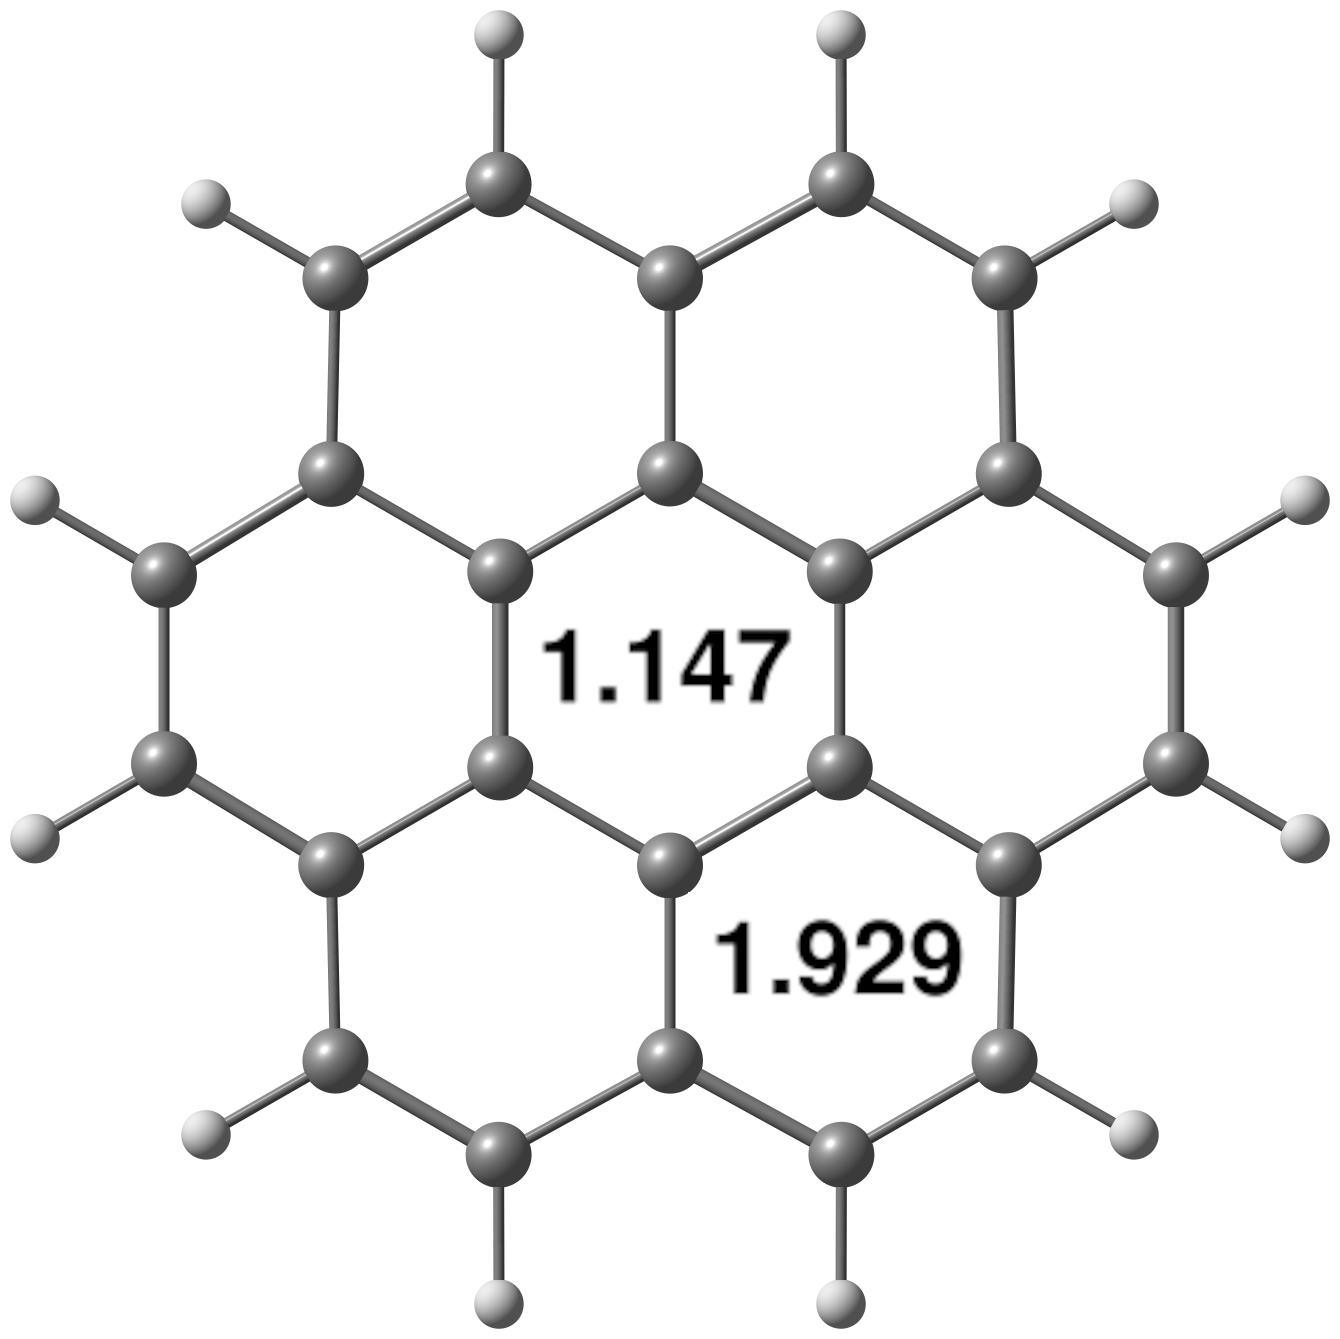
\includegraphics[width=\textwidth]{./figures/coronene-giamb}
			\caption{{\small Giambiagi 6-delocalization index results in au and multiplied by \num{e-4}.}}
			\label{fig:CoroneneGiamb}
		\end{subfigure}
		~ %add desired spacing between images, e. g. ~, \quad, \qquad, \hfill etc. 
		%(or a blank line to force the subfigure onto a new line)
		\begin{subfigure}[b]{0.4\textwidth}
			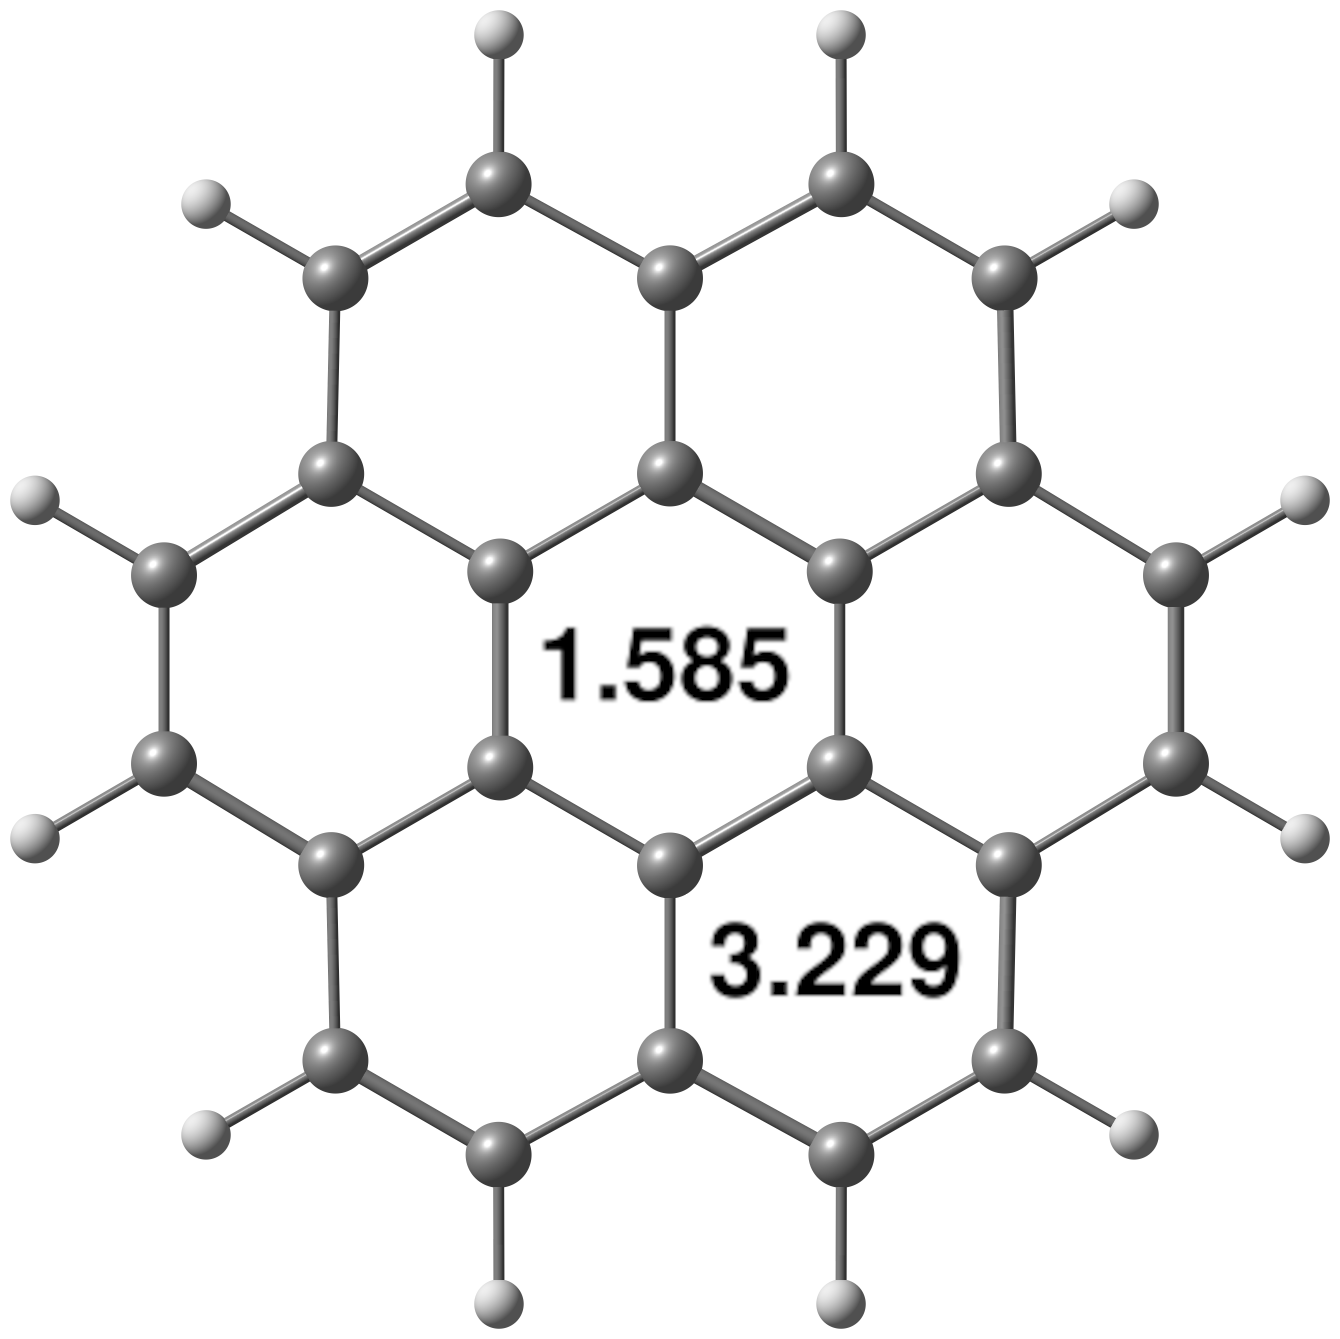
\includegraphics[width=\textwidth]{./figures/coronene-ponec}
			\caption{{\small Ponec 6-delocalization index results in au and multiplied by \num{e-3}.}}
			\label{fig:CoronenePonec}
		\end{subfigure}
		\caption{\ac{FOHI} Giambiagi (left) and Ponec (right) 6-delocalization indices for the symmetrically-independent rings of the coronene molecule at B3LYP/6-31G(d,p).}\label{fig:Coronene6Dec}
	\end{figure}
\end{center}

The first part of the output file consists of a computational details summary. Concretely, the input file name the calculation comes from, the wave function file and some molecular parameters such as the wave function type (restricted or unrestricted), the number of \acp{MO}, the number of basis functions and the total number of (heavy) atoms are included here:
\begin{recuadro}{Header, input and wave functions files together with some molecular parameters}
+++++++++++++++++++++++++++++++++++++
        N D E L O C  v.1.2.17
+++++++++++++++++++++++++++++++++++++
+ 6-(DE)LOC calculation :  coronene +
+++++++++++++++++++++++++++++++++++++
>> SUMMARY :
* INPUT file ............ coronene-6delpi.ndinp
* FCHK   file ........... coronene.fchk
* NMO,NBFUNC,NAtoms ..... 78, 420, 36 (Restricted)
* # Heavy atoms ......... 24
\end{recuadro}
In the case of PROAIMS wave function (.wfn) and MOLDEN (.molden) files, \programa~ will print, in addition, the number of primitive functions and the type of the wave function (HF/KS or post-HF/2hybrid KS).

Next, the \acp{MO} selected by the user in a compact way (see \autoref{sec:line3} for more details), the index order of the calculation and whether the localization indices were computed (option available if the index order is greater than 2) (see \autoref{sec:line4} for more details):
\begin{recuadro}{Set of \acp{MO}}
* Specified orbitals .... 55,61-62,68-69,72-78 PI(12)
* (DE)LOC index order ... 6
* LOC indices included .. NO (Available if N>2)
* # (DE)LOC indices ..... 2 (LOC+DELOC)
\end{recuadro}
Moreover, the program prints how many calculations have been computed.

In the case of post-HF wave functions, and if there are occupation numbers  tending to be negligible, the program will truncate the set of \acp{MO}, printing a message in the output file. If the scaling of post-HF \acp{AOM} or \acp{BOM} is activated, a message will be included as well.

The type of overlap matrices is the next information printed in the output. If the calculation employed \acfp{AOM}, then the corresponding notification is added in the output together with atoms considered in the calculation in a compact way. Otherwise, a message about the use of \acfp{BOM} is included.
\begin{recuadro}{Type of overlap matrix and the participating atoms/basins}
* Atomic overlap matrices (AOM) employed *
* Considered atoms ...... 1-10 (10)
\end{recuadro}
When the ring perception is set (see \autoref{sec:line5} for more details) \programa~ includes the number of rings detected by the algorithm and the bond length cut-off, \emph{i.e.}, the limit to distinguish between a pair of bonded atoms or another type of distance. In the case of including the \emph{xyz} option in Line~2 (see \autoref{sec:line2} for more details) and the index order is greater than 2, the program creates one (if \emph{giamb} label is added in Line~4, see \autoref{sec:line4}) or two .xyz files and prints a notification in the main output file.
\begin{recuadro}{Ring perception and xyz files}
* # detected rings ...... 2
* Bond dist cut-off ..... 1.600
* XYZ Files with DELOC .. YES
\end{recuadro}

The next step of the output file will show the \ac{AOM} or \ac{BOM} files used by the program:
\begin{recuadro}{\ac{AOM} or \ac{BOM} files}
>> FILES   :
* AOM File   1 .......... coronene_coronene_C001.fuk
* AOM File   2 .......... coronene_coronene_C002.fuk
[...]
* AOM File  10 .......... coronene_coronene_C010.fuk
\end{recuadro}

If the \emph{xyz} option is correctly set, the program will print the names of the .xyz files and the multiplication factor of the indices. Keep in mind if the calculation only includes the Giambiagi approach, only the Giambiagi approach file is generated.
\begin{recuadro}{.xyz output file names}
Multiplication factors (gia,pon): 10000,1000
* XYZ File .............. coronene-6delpi-ndel6-gia.xyz
* XYZ File .............. coronene-6delpi-ndel6-pon.xyz
\end{recuadro}

The last section of the output file will evidently include the results together with the numbering of the atoms/basins considered. Two kinds of normalizations are also printed to make comparable the results with other values from different index order.
\begin{recuadro}{Results}
>> RESULTS :
coronene 6-DELOC :                                        Giambiagi      Ponec
* Index   1 ............. C001 C002 C003 C004 C005 C006   1.929E-04  3.229E-03
-        Ponec's norm.                                    6.174E-03  1.033E-01
- Cioslowski's norm.                                      2.404E-01  3.844E-01
* Index   2 ............. C003 C004 C008 C009 C010 C007   1.147E-04  1.585E-03
-      Ponec's norm.                                      3.672E-03  5.072E-02
- Cioslowski's norm.                                      2.204E-01  3.415E-01
\end{recuadro}

Finally, the overall elapsed and the most computationally demanding partial times are included:
\begin{recuadro}{Elapsed time}
>> qcksort spent ........... 0.00 seconds
>> Connect analysis spent .. 0.00 seconds
>> Elapsed time ............ 0.25 seconds
\end{recuadro}

\section[Output file when $N=2$]{Output file when the index order corresponds to $N=2$}\label{sec:outputNeq2}
In this section we will discuss the differences between the general output file, when the index order is greater than two (\autoref{sec:outputNgt2}), and the 2-order calculation. Consider the following input file:
\begin{consola}{cat coronene-2de-loc.ndinp}
coronene.fchk 4
coronene-2de-loc
pi
2
all
fuk
\end{consola}
The main changed part corresponds to the {\texttt{RESULTS}} (the \texttt{SUMMARY} structure of the computational details is kept unaltered). There, \programa~ prints
 both localization and delocalization indices as diagonal and off-diagonal elements of a triangular matrix, respectively (useful to be opened with a spreadsheet software, such as M\$ Excel or Libreoffice Calc).
\begin{recuadro}{Fragment of the triangular matrix of 2-(de)localization indices for coronene}
>> RESULTS :
                   C001       C002       C003       [...]
coronene  C001     0.37077
coronene  C002     0.28676    0.32624
coronene  C003     0.05361    0.29211    0.34398
[...]
\end{recuadro}
The localization indices correspond to the electron population not shared by the atoms while the 2-delocalization values represent the quantity of electrons partaken by two atoms. Normally, if the atoms are directly neighbors, the index is interpreted as the \emph{bond order}. Otherwise, they can be used to analyze mesomeric/resonance effects.

Inasmuch as the triangular matrix can be ``uncomfortable'' to find a specific value, \programa~ prints the localization indices for each atom the user has requested in a separated block:
\begin{recuadro}{Block of 2-localization indices}
LOC :
C001    0.37077
C002    0.32624
C003    0.34398
C004    0.34400
C005    0.32622
[...]
\end{recuadro}
The next block is evidently formed by all the 2-delocalization indices\footnote{We have added the text ``BOND ORDER'' to remark these values on purpose but \programa~ does not have this feature currently.}:
\begin{recuadro}{Block of 2-delocalization indices}
DELOC :
1     2    0.28676    << BOND ORDER
1     3    0.05361
1     4    0.04550
1     5    0.06649
1     6    0.49491    << BOND ORDER
1     7    0.00485
1     8    0.00635
\end{recuadro}

Finally, the elapsed time is also included:
\begin{recuadro}{Elapsed time}
>> Elapsed time ............ 0.07 seconds
\end{recuadro}

%\chapter{Examples}
%
%\chapter{GNU/Linux benchmarks}
%

\backmatter % Back matter begins
%
\printbibliography
%
%\begin{appendices} 
%\chapter{Appendices}
%\section{Obtaining PROAIMS wave function file}\label{appx:getwfn}
%\end{appendices}

\vspace{7cm}

\begin{center}
	\begin{tabular}{c@{\hspace{3cm}}c}
		Nicolás Otero Martínez & Marcos Mandado Alonso
	\end{tabular}
\end{center}

\end{document}
